
%% bare_jrnl_compsoc.tex
%% V1.4b
%% 2015/08/26
%% by Michael Shell
%% See:
%% http://www.michaelshell.org/
%% for current contact information.
%%
%% This is a skeleton file demonstrating the use of IEEEtran.cls
%% (requires IEEEtran.cls version 1.8b or later) with an IEEE
%% Computer Society journal paper.
%%
%% Support sites:
%% http://www.michaelshell.org/tex/ieeetran/
%% http://www.ctan.org/pkg/ieeetran
%% and
%% http://www.ieee.org/

%%*************************************************************************
%% Legal Notice:
%% This code is offered as-is without any warranty either expressed or
%% implied; without even the implied warranty of MERCHANTABILITY or
%% FITNESS FOR A PARTICULAR PURPOSE! 
%% User assumes all risk.
%% In no event shall the IEEE or any contributor to this code be liable for
%% any damages or losses, including, but not limited to, incidental,
%% consequential, or any other damages, resulting from the use or misuse
%% of any information contained here.
%%
%% All comments are the opinions of their respective authors and are not
%% necessarily endorsed by the IEEE.
%%
%% This work is distributed under the LaTeX Project Public License (LPPL)
%% ( http://www.latex-project.org/ ) version 1.3, and may be freely used,
%% distributed and modified. A copy of the LPPL, version 1.3, is included
%% in the base LaTeX documentation of all distributions of LaTeX released
%% 2003/12/01 or later.
%% Retain all contribution notices and credits.
%% ** Modified files should be clearly indicated as such, including  **
%% ** renaming them and changing author support contact information. **
%%*************************************************************************


% *** Authors should verify (and, if needed, correct) their LaTeX system  ***
% *** with the testflow diagnostic prior to trusting their LaTeX platform ***
% *** with production work. The IEEE's font choices and paper sizes can   ***
% *** trigger bugs that do not appear when using other class files.       ***                          ***
% The testflow support page is at:
% http://www.michaelshell.org/tex/testflow/


\documentclass[10pt,journal,compsoc]{IEEEtran}
%
% If IEEEtran.cls has not been installed into the LaTeX system files,
% manually specify the path to it like:
% \documentclass[10pt,journal,compsoc]{../sty/IEEEtran}




%Todd packages and commands
\usepackage[normalem]{ulem} %for sout  
\usepackage[all]{nowidow} %for no orphan lines
\newcommand{\strikeout}[1]{\sout{#1}}
\newcommand{\quotes}[1]{``#1''}
\newcommand{\emphasis}[1]{\emph{#1}}

\newcommand{\participantQuote}[1]{\textit{``#1''}}
\newcommand{\oneColumnWidth}{3.4in}
\newcommand{\twoColumnWidth}{7.1in}
\usepackage{caption} %for lableling a table as a figure
\newcommand{\numberOfObservedProjects}{eight}
\newcommand{\numberOfInterviews}{33}
\newcommand{\durationOfResearchStudy}{two-year five-month}
\newcommand{\durationOfResearchStudyPlural}{two-years and five-months}
\usepackage[disable]{todonotes} % notes not showed

% http://tex.stackexchange.com/questions/12703/how-to-create-fixed-width-table-columns-with-text-raggedright-centered-raggedlef
\usepackage{array}
%\newcolumntype{L}[1]{>{\raggedright\let\newline\\\arraybackslash\hspace{0pt}}m{#1}}
%\newcolumntype{C}[1]{>{\centering\let\newline\\\arraybackslash\hspace{0pt}}m{#1}}
%\newcolumntype{R}[1]{>{\raggedleft\let\newline\\\arraybackslash\hspace{0pt}}m{#1}}
% \newcolumntype{LEFT}[1]{>{\raggedright\arraybackslash}p{#1}}



% Some very useful LaTeX packages include:
% (uncomment the ones you want to load)


% *** MISC UTILITY PACKAGES ***
%
%\usepackage{ifpdf}
% Heiko Oberdiek's ifpdf.sty is very useful if you need conditional
% compilation based on whether the output is pdf or dvi.
% usage:
% \ifpdf
%   % pdf code
% \else
%   % dvi code
% \fi
% The latest version of ifpdf.sty can be obtained from:
% http://www.ctan.org/pkg/ifpdf
% Also, note that IEEEtran.cls V1.7 and later provides a builtin
% \ifCLASSINFOpdf conditional that works the same way.
% When switching from latex to pdflatex and vice-versa, the compiler may
% have to be run twice to clear warning/error messages.






% *** CITATION PACKAGES ***
%
\ifCLASSOPTIONcompsoc
  % IEEE Computer Society needs nocompress option
  % requires cite.sty v4.0 or later (November 2003)
  \usepackage[nocompress]{cite}
\else
  % normal IEEE
  \usepackage{cite}
\fi
% cite.sty was written by Donald Arseneau
% V1.6 and later of IEEEtran pre-defines the format of the cite.sty package
% \cite{} output to follow that of the IEEE. Loading the cite package will
% result in citation numbers being automatically sorted and properly
% "compressed/ranged". e.g., [1], [9], [2], [7], [5], [6] without using
% cite.sty will become [1], [2], [5]--[7], [9] using cite.sty. cite.sty's
% \cite will automatically add leading space, if needed. Use cite.sty's
% noadjust option (cite.sty V3.8 and later) if you want to turn this off
% such as if a citation ever needs to be enclosed in parenthesis.
% cite.sty is already installed on most LaTeX systems. Be sure and use
% version 5.0 (2009-03-20) and later if using hyperref.sty.
% The latest version can be obtained at:
% http://www.ctan.org/pkg/cite
% The documentation is contained in the cite.sty file itself.
%
% Note that some packages require special options to format as the Computer
% Society requires. In particular, Computer Society  papers do not use
% compressed citation ranges as is done in typical IEEE papers
% (e.g., [1]-[4]). Instead, they list every citation separately in order
% (e.g., [1], [2], [3], [4]). To get the latter we need to load the cite
% package with the nocompress option which is supported by cite.sty v4.0
% and later. Note also the use of a CLASSOPTION conditional provided by
% IEEEtran.cls V1.7 and later.





% *** GRAPHICS RELATED PACKAGES ***
%
\ifCLASSINFOpdf
  % \usepackage[pdftex]{graphicx}
  % declare the path(s) where your graphic files are
  % \graphicspath{{../pdf/}{../jpeg/}}
  % and their extensions so you won't have to specify these with
  % every instance of \includegraphics
  % \DeclareGraphicsExtensions{.pdf,.jpeg,.png}
\else
  % or other class option (dvipsone, dvipdf, if not using dvips). graphicx
  % will default to the driver specified in the system graphics.cfg if no
  % driver is specified.
  % \usepackage[dvips]{graphicx}
  % declare the path(s) where your graphic files are
  % \graphicspath{{../eps/}}
  % and their extensions so you won't have to specify these with
  % every instance of \includegraphics
  % \DeclareGraphicsExtensions{.eps}
\fi
% graphicx was written by David Carlisle and Sebastian Rahtz. It is
% required if you want graphics, photos, etc. graphicx.sty is already
% installed on most LaTeX systems. The latest version and documentation
% can be obtained at: 
% http://www.ctan.org/pkg/graphicx
% Another good source of documentation is "Using Imported Graphics in
% LaTeX2e" by Keith Reckdahl which can be found at:
% http://www.ctan.org/pkg/epslatex
%
% latex, and pdflatex in dvi mode, support graphics in encapsulated
% postscript (.eps) format. pdflatex in pdf mode supports graphics
% in .pdf, .jpeg, .png and .mps (metapost) formats. Users should ensure
% that all non-photo figures use a vector format (.eps, .pdf, .mps) and
% not a bitmapped formats (.jpeg, .png). The IEEE frowns on bitmapped formats
% which can result in "jaggedy"/blurry rendering of lines and letters as
% well as large increases in file sizes.
%
% You can find documentation about the pdfTeX application at:
% http://www.tug.org/applications/pdftex






% *** MATH PACKAGES ***
%
%\usepackage{amsmath}
% A popular package from the American Mathematical Society that provides
% many useful and powerful commands for dealing with mathematics.
%
% Note that the amsmath package sets \interdisplaylinepenalty to 10000
% thus preventing page breaks from occurring within multiline equations. Use:
%\interdisplaylinepenalty=2500
% after loading amsmath to restore such page breaks as IEEEtran.cls normally
% does. amsmath.sty is already installed on most LaTeX systems. The latest
% version and documentation can be obtained at:
% http://www.ctan.org/pkg/amsmath





% *** SPECIALIZED LIST PACKAGES ***
%
%\usepackage{algorithmic}
% algorithmic.sty was written by Peter Williams and Rogerio Brito.
% This package provides an algorithmic environment fo describing algorithms.
% You can use the algorithmic environment in-text or within a figure
% environment to provide for a floating algorithm. Do NOT use the algorithm
% floating environment provided by algorithm.sty (by the same authors) or
% algorithm2e.sty (by Christophe Fiorio) as the IEEE does not use dedicated
% algorithm float types and packages that provide these will not provide
% correct IEEE style captions. The latest version and documentation of
% algorithmic.sty can be obtained at:
% http://www.ctan.org/pkg/algorithms
% Also of interest may be the (relatively newer and more customizable)
% algorithmicx.sty package by Szasz Janos:
% http://www.ctan.org/pkg/algorithmicx




% *** ALIGNMENT PACKAGES ***
%
%\usepackage{array}
% Frank Mittelbach's and David Carlisle's array.sty patches and improves
% the standard LaTeX2e array and tabular environments to provide better
% appearance and additional user controls. As the default LaTeX2e table
% generation code is lacking to the point of almost being broken with
% respect to the quality of the end results, all users are strongly
% advised to use an enhanced (at the very least that provided by array.sty)
% set of table tools. array.sty is already installed on most systems. The
% latest version and documentation can be obtained at:
% http://www.ctan.org/pkg/array


% IEEEtran contains the IEEEeqnarray family of commands that can be used to
% generate multiline equations as well as matrices, tables, etc., of high
% quality.




% *** SUBFIGURE PACKAGES ***
%\ifCLASSOPTIONcompsoc
%  \usepackage[caption=false,font=footnotesize,labelfont=sf,textfont=sf]{subfig}
%\else
%  \usepackage[caption=false,font=footnotesize]{subfig}
%\fi
% subfig.sty, written by Steven Douglas Cochran, is the modern replacement
% for subfigure.sty, the latter of which is no longer maintained and is
% incompatible with some LaTeX packages including fixltx2e. However,
% subfig.sty requires and automatically loads Axel Sommerfeldt's caption.sty
% which will override IEEEtran.cls' handling of captions and this will result
% in non-IEEE style figure/table captions. To prevent this problem, be sure
% and invoke subfig.sty's "caption=false" package option (available since
% subfig.sty version 1.3, 2005/06/28) as this is will preserve IEEEtran.cls
% handling of captions.
% Note that the Computer Society format requires a sans serif font rather
% than the serif font used in traditional IEEE formatting and thus the need
% to invoke different subfig.sty package options depending on whether
% compsoc mode has been enabled.
%
% The latest version and documentation of subfig.sty can be obtained at:
% http://www.ctan.org/pkg/subfig




% *** FLOAT PACKAGES ***
%
%\usepackage{fixltx2e}
% fixltx2e, the successor to the earlier fix2col.sty, was written by
% Frank Mittelbach and David Carlisle. This package corrects a few problems
% in the LaTeX2e kernel, the most notable of which is that in current
% LaTeX2e releases, the ordering of single and double column floats is not
% guaranteed to be preserved. Thus, an unpatched LaTeX2e can allow a
% single column figure to be placed prior to an earlier double column
% figure.
% Be aware that LaTeX2e kernels dated 2015 and later have fixltx2e.sty's
% corrections already built into the system in which case a warning will
% be issued if an attempt is made to load fixltx2e.sty as it is no longer
% needed.
% The latest version and documentation can be found at:
% http://www.ctan.org/pkg/fixltx2e


%\usepackage{stfloats}
% stfloats.sty was written by Sigitas Tolusis. This package gives LaTeX2e
% the ability to do double column floats at the bottom of the page as well
% as the top. (e.g., "\begin{figure*}[!b]" is not normally possible in
% LaTeX2e). It also provides a command:
%\fnbelowfloat
% to enable the placement of footnotes below bottom floats (the standard
% LaTeX2e kernel puts them above bottom floats). This is an invasive package
% which rewrites many portions of the LaTeX2e float routines. It may not work
% with other packages that modify the LaTeX2e float routines. The latest
% version and documentation can be obtained at:
% http://www.ctan.org/pkg/stfloats
% Do not use the stfloats baselinefloat ability as the IEEE does not allow
% \baselineskip to stretch. Authors submitting work to the IEEE should note
% that the IEEE rarely uses double column equations and that authors should try
% to avoid such use. Do not be tempted to use the cuted.sty or midfloat.sty
% packages (also by Sigitas Tolusis) as the IEEE does not format its papers in
% such ways.
% Do not attempt to use stfloats with fixltx2e as they are incompatible.
% Instead, use Morten Hogholm'a dblfloatfix which combines the features
% of both fixltx2e and stfloats:
%
% \usepackage{dblfloatfix}
% The latest version can be found at:
% http://www.ctan.org/pkg/dblfloatfix




%\ifCLASSOPTIONcaptionsoff
%  \usepackage[nomarkers]{endfloat}
% \let\MYoriglatexcaption\caption
% \renewcommand{\caption}[2][\relax]{\MYoriglatexcaption[#2]{#2}}
%\fi
% endfloat.sty was written by James Darrell McCauley, Jeff Goldberg and 
% Axel Sommerfeldt. This package may be useful when used in conjunction with 
% IEEEtran.cls'  captionsoff option. Some IEEE journals/societies require that
% submissions have lists of figures/tables at the end of the paper and that
% figures/tables without any captions are placed on a page by themselves at
% the end of the document. If needed, the draftcls IEEEtran class option or
% \CLASSINPUTbaselinestretch interface can be used to increase the line
% spacing as well. Be sure and use the nomarkers option of endfloat to
% prevent endfloat from "marking" where the figures would have been placed
% in the text. The two hack lines of code above are a slight modification of
% that suggested by in the endfloat docs (section 8.4.1) to ensure that
% the full captions always appear in the list of figures/tables - even if
% the user used the short optional argument of \caption[]{}.
% IEEE papers do not typically make use of \caption[]'s optional argument,
% so this should not be an issue. A similar trick can be used to disable
% captions of packages such as subfig.sty that lack options to turn off
% the subcaptions:
% For subfig.sty:
% \let\MYorigsubfloat\subfloat
% \renewcommand{\subfloat}[2][\relax]{\MYorigsubfloat[]{#2}}
% However, the above trick will not work if both optional arguments of
% the \subfloat command are used. Furthermore, there needs to be a
% description of each subfigure *somewhere* and endfloat does not add
% subfigure captions to its list of figures. Thus, the best approach is to
% avoid the use of subfigure captions (many IEEE journals avoid them anyway)
% and instead reference/explain all the subfigures within the main caption.
% The latest version of endfloat.sty and its documentation can obtained at:
% http://www.ctan.org/pkg/endfloat
%
% The IEEEtran \ifCLASSOPTIONcaptionsoff conditional can also be used
% later in the document, say, to conditionally put the References on a 
% page by themselves.




% *** PDF, URL AND HYPERLINK PACKAGES ***
%
%\usepackage{url}
% url.sty was written by Donald Arseneau. It provides better support for
% handling and breaking URLs. url.sty is already installed on most LaTeX
% systems. The latest version and documentation can be obtained at:
% http://www.ctan.org/pkg/url
% Basically, \url{my_url_here}.





% *** Do not adjust lengths that control margins, column widths, etc. ***
% *** Do not use packages that alter fonts (such as pslatex).         ***
% There should be no need to do such things with IEEEtran.cls V1.6 and later.
% (Unless specifically asked to do so by the journal or conference you plan
% to submit to, of course. )


% correct bad hyphenation here
\hyphenation{op-tical net-works semi-conduc-tor}


\begin{document}


% Sample apostrophy’s to remove team’s 

\title{Sustainable Software Development through Overlapping Pair Rotation}

\author{Todd~Sedano,~\IEEEmembership{Member,~IEEE,}
        Paul~Ralph,~\IEEEmembership{Member,~IEEE,}
        and~C\'ecile~P\'eraire,~\IEEEmembership{Member,~IEEE}% <-this % stops a space
\IEEEcompsocitemizethanks{\IEEEcompsocthanksitem T. Sedano was with Pivotal Software and with the Department of Electrical and Computer Engineering, Carnegie Mellon University, Pittsburgh,
CA, 15412.\protect\\
% note need leading \protect in front of \\ to get a newline within \thanks as
% \\ is fragile and will error, could use \hfil\break instead.
E-mail: professor@gmail.com
\IEEEcompsocthanksitem P. Raul is with University of Auckland, 
  Auckland, New Zealand and University of British Columbia, Vancouver, BC, Canada.
E-mail: paul@paulralph.name
\IEEEcompsocthanksitem C.  P\'eraire is with the  Department of Electrical and Computer Engineering, Carnegie Mellon University, Silicon Valley Campus, Moffett Field, CA
E-mail: cecile.peraire@sv.cmu.edu
}% <-this % stops an unwanted space

\thanks{Manuscript received April 19, 2005; revised August 26, 2015.}}

\markboth{Journal of \LaTeX\ Class Files,~Vol.~14, No.~8, August~2015}%
{Shell \MakeLowercase{\textit{et al.}}: Bare Demo of IEEEtran.cls for Computer Society Journals}

\IEEEtitleabstractindextext{%
\begin{abstract}

\textit{Context:} Conventional wisdom says that team disruptions (like team churn) should be avoided. However, we have observed software development projects that succeed despite high disruption. 

\textit{Objective:} The purpose of this paper is to understand how to develop software effectively, even in the face of team disruption.

\textit{Method:} We followed Constructivist Grounded Theory. We conducted participant-observation of several projects at Pivotal (a software development company), and interviewed 21 software engineers, interaction designers, and product managers. The researchers iteratively sampled and analyzed the collected data until achieving theoretical saturation.

\textit{Results:} This paper introduces a descriptive theory of Sustainable Software Development. The theory encompasses principles, policies, and practices aiming at removing knowledge silos and improving code quality (including discoverability and readability), hence leading to development sustainability. 

\textit{Limitations:} While the results are highly relevant to the observed projects at Pivotal, the outcomes may not be transferable to other software development organizations with different software development cultures.

\textit{Conclusion:} The theory refines and extends our understanding of Extreme Programming by adding new principles, policies, and practices (including Overlapping Pair Rotation) and aligning them with the business goal of sustainability. 

\end{abstract}
\begin{IEEEkeywords}
Computer Society, IEEE, IEEEtran, journal, \LaTeX, paper, template.
\end{IEEEkeywords}
}

\maketitle

\IEEEdisplaynontitleabstractindextext
\IEEEpeerreviewmaketitle

\IEEEraisesectionheading{\section{Introduction}\label{sec:introduction}}

\section{Introduction}
\IEEEPARstart{I}{magine} being a software development manager when one of your top engineers, Dakota, gives notice and is moving on to a new job opportunity. You are simultaneously excited because the new position provides a great career opportunity for someone you respect, yet distressed that her departure may exacerbate your own project. How will the team overcome this disruption? Your investment in this engineer and her entire accumulated knowledge about the project is evaporating. Dakota developed some of the systems' trickiest, most important components. How long will it take the other programmers to assimilate Dakota's code?  How will this affect their productivity and future development?


Conventional wisdom says that team churn is detrimental to project success and that extensive documentation is needed to mitigate this effect. Unfortunately, documentation quickly becomes out-of-date and unreliable \cite{Lethbridge2003Documentation}, undermining this approach. During a Grounded Theory study, we observed projects succeed despite high disruption and little documentation. This raised the following research question: \quotes{How do the observed teams develop software effectively while overcoming team disruption?}

Exploring this question resulted in a descriptive theory of \quotes{Sustainable Software Development.} The theory explains how a collection of synergistic principles, policies, and practices help develop software effectively while overcoming team disruption. This is done by engendering a positive attitude towards team disruption, encouraging knowledge sharing and continuity, as well as prioritizing high code quality. Here, \textit{team disruption} refers to substantial ongoing changes in team composition, including team members joining or leaving, as well as temporary vacations or leave of absence. 

In Section \ref{RelatedWork}, we present related work on Extreme Programming and team disruption. In Section \ref{ResearchMethod}, we review how we employed Constructivist Grounded Theory to derive a descriptive theory supported by empirical data. We also present the research context, introducing both the company and one of the five projects under study. In Section \ref{Theory}, we describe the theory and how its principles, policies, and practices work together to achieve software development sustainability. In Section \ref{TheoryEvaluation}, we evaluate the theory using established criteria for evaluating a Grounded Theory. In the last sections, we examine threats to research validity, consider future research, and conclude the research.
\section{Related Work}
\label{RelatedWork}
In Extreme Programming \cite{BeckExtremeProgramming2004}, Kent Beck describes a set of interdependent practices that manage feature development (much like Scrum \cite{SchwaberScrum}), as well as technical practices that facilitate a collaborative team environment. Extreme Programming comprises 13 primary practices and 11 corollary practices. 

One Extreme Programming practice, collective ownership, simply means that \quotes{anyone on the team can improve any part of the system at any time.} Beck contrasts collective ownership with \quotes{no ownership} and \quotes{individual ownership.} With collective ownership, every developer takes responsibility for the whole of the system. When developers see opportunities to improve the code, they go ahead and improve it if it makes their life easier \cite{BeckExtremeProgramming1999}. Later, \quotes{collective ownership} was renamed to \quotes{shared code} \cite{BeckExtremeProgramming2004}. 

One Extreme Programming practice contributing to collective code ownership is pair programming. Pair programming is where production code is created by two developers working together at a single computer \cite{BeckExtremeProgramming2004}. Extreme Programming does not prescribe how pairs are formed or for how long a pair works together. Williams presents a pair rotation strategy for maintaining specialization, by \quotes{choosing the right partner for the right situation}  \cite{Williams2002}. People are assigned modules of the code to own based upon expertise and find partners from neighboring modules. While knowledge is shared with pairing, one person owns every story that touches their part of the system, building individual code ownership. In one case study, the project started with a pair rotation strategy based on skillsets but evolved into a daily rotation determined randomly \cite{Vanhanen2007}. Some teams use a pair programing matrix \cite{AlaverdyanPairProgrammingMatrix} (also called a pairing ladder \cite{Davies2009AgileCoaching}) to track who has paired with whom for the purpose of pairing people who have not paired recently.

Truck Number is \quotes{The size of the smallest set of people in a project such that, if all of them got hit by a truck, the project would be in trouble.} \cite{WikiTruckNumber}. Truck Number, or Bus Count, reminds management about the effects of disruptive events for a team. In 1994, Coplien \cite{Coplien1994} mentions \quotes{Truck Number} as a risk to his Solo Virtuoso pattern of using only one talented developer to create a software system. Awati suggests that Truck Number can be increased by reducing complexity, cross-training, and documentation \cite{AwatiBusFactor}, all of which are found in Extreme Programming. However, Extreme Programming implements \quotes{documentation} as discoverable, intention revealing code. Ricca \cite{Ricca2011TruckFactor} examines the difficulty in computing the Truck Number. 

Rigby quantifies turnover using knowledge at risk analysis on abandoned files  \cite{Rigby2016Turnover}. A line of code is abandoned if the most recent contributor has left the company.  A file is abandoned if more than 90\% of the lines in the file are abandoned.  Izquierdo examines how teams managed orphaned code \cite{Izquierdo2009Turnover}. Joseph examines job turnovers to understand the reasons developers leave their company  \cite{Joseph2007Turnover}.  
\section{Research Method}
\label{ResearchMethod}
\subsection{Constructivist Grounded Theory}

We adopted Grounded Theory \cite{Charmaz}, which provides an iterative approach to data collection, data coding, and analysis resulting in an emergent theory. We selected Charmaz' Constructivist approach to Grounded Theory, which \quotes{emphasizes understanding and acknowledges that data, interpretations, and resulting theory depend on the researcher’s view} \cite{StolGroundedTheory}. The two primary data sources were field notes collected during continuous participant observations of a seven-month project and interviews with Pivotal software engineers, interaction designers, and product managers. Interviews were recorded, transcribed, coded, and analyzed using constant comparison. In addition, the first author was involved in four other projects as participant-observer.

Grounded Theory immerses the researcher within the context of the research subject from the point of view of the participants. As the research progresses, Grounded Theory allows the researcher to \quotes{incrementally direct the data collection and theoretical ideas.} The theory provides a starting place for inquiry, not a specific goal known at the beginning of the research. As we interact with the data, the data influence how we progress and alter the research direction. When starting a Grounded Theory research study, the core question is, \quotes{What is happening here?} \cite{GlaserTheoreticalSensitivity}. Our initial core question was \quotes{What is happening at Pivotal when it comes to software development?}
\subsection{Participants}
The first author interviewed 21 interaction designers, product managers, and software engineers who had experience with Pivotal's software development process. They were distributed across four different Pivotal offices. Interaction designers identify user needs predominately through user interviews; create and validate user experience with mockups; determine the visual design of a product; and support engineering during implementation. Product managers are responsible for identifying and prioritizing features, converting features into stories, prioritizing stories in a backlog, and communicating the stories to the engineers. Software engineers implement the solution. Participants were not paid for their time. 
\subsection{Data Collection}
We relied on \quotes{intensive interviews,} which are \quotes{open-ended yet directed, shaped yet emergent, and paced yet unrestricted} \cite{Charmaz}. Open-ended questions were used to enter into the participant's personal perspective within the context of the research question. The interviewer attempts to abandon assumptions to better understand and explore the interviewee's perspective. Charmaz \cite{Charmaz} contrasts intensive interviews from informational interviews, which facilitate collecting accurate `facts’ and investigative interviews that attempt to reveal hidden intentions or expose practices and policies. 
 
The initial interviews were open-ended explorations starting with the question, \quotes{Please draw on this sheet of paper your view of Pivotal's software development process.} The interviewer specifically did not force initial topics and merely followed the path of the interviewee. 

While exploring new emergent core categories, whenever possible, subsequent interviews were initiated with open-ended questions.  For example, asking the participant, \quotes{Please draw your feelings about the code} often resulted in conversations about code ownership. 

Each interview was transcribed into a Word document with timecode stamps for each segment.

In addition to collecting data from interviews, the first author collected field notes while working as an engineer on the project described in Section \ref{ProjectQuattuor}. The field notes comprised multiple paragraph entries recorded several times a week, collected over seven months. These notes described individual and collective actions, captured what participants defined as interesting or problematic, and included anecdotes and observations. 
\subsection{Data Analysis}
Data analysis began with line-by-line coding as recommended by Charmaz \cite{Charmaz}. Coding line-by-line helps the researcher identify nuanced interactions in the data and avoid jumping to conclusions. The data then advanced from these initial codes to focused codes, focused codes to core categories, and core categories to an emergent theory. 

We reviewed the initial codes while reading the transcripts and listening to the audio recordings. We discussed the coding during weekly research collaboration meetings. To avoid missing insights from these discussions \cite{GlaserTheoreticalSensitivity}, we recorded and transcribed them into grounded theory memos. 

As data was collected and coded, we recorded initial codes in a spreadsheet and we used constant comparison to generate focused codes. Only ideas expressed by multiple interviewees informed focused codes and subsequent analysis.

We constantly compared new codes to existing codes to refine codes and eventually generate categories. We periodically audited each category for cohesion by comparing its codes. When this became complex, the codes were printed on index cards, and then arranged and re-arranged until cohesive categories emerged. We wrote memos to capture the analysis of codes, examinations of theoretical plausibility, and insights. 

Constant comparison allowed us to identify \quotes{the conceptual relationship between categories and their properties as they emerged} \cite{GlaserBasics}, leading to a resulting descriptive theory. The resulting theory is presented in Section \ref{Theory} and illustrated in Table \ref{SustainableSoftwareDevelopmentTable}. The table includes the main categories and their organization into principles, policies, and practices. Examples of quotes leading to some categories are presented in Table \ref{ChainOfEvidenceTable}.


\begin{table}[t]
\renewcommand{\arraystretch}{1.5}
\centering
\caption{Quotes for Selected Categories}
\label{ChainOfEvidenceTable}
\begin{tabular}{|p{3.15in}|}
\hline
Engendering Positive Attitudes Toward Team Disruption \\
\hline
\participantQuote{I'm excited when a new person joins the team. That person has experience that might add something to the project.} \\

\participantQuote{I like that people bring new energy. Projects often get into the state of a lull with the same people working on it and have the same cadence. New people bring a new perspective. [Two engineers recently joined] and it was really cool to see their fresh perspective. I always like people joining a project.} \\

\participantQuote{Team members go out of their way to make new teammates feel welcome and help ramp them up.} \\

\hline
Team Code Ownership \\
\hline
\participantQuote{I feel ownership of the code as a whole, and I feel empowered and able to go and work on any part of the codebase.} \\
\participantQuote{I don't feel like I have [individual] ownership. It's really a collaborative effort to achieve where we are today \ldots I feel like everybody owns this product.} \\
\participantQuote{There is a lot of emphasis that you are not your code.} \\
\participantQuote{I never feel like a specific piece is mine or something belongs to other people.}\\

\hline
Overlapping Pair Rotation \\
\hline
\participantQuote{To make sure that knowledge silos don't form we rotate pairs. As people work on specific stories and specific parts of the code, we want to share that knowledge.} \\

\participantQuote{Rotating pairs reduces knowledge silos and reduces the bus factor. We do not want the departure of one developer from the project to cripple the project.} \\

\participantQuote{We rotate pairs because everyone has a different set of knowledge. When you work with someone you get a little bit of that knowledge. The more you pair with them, the more knowledge you get.} \\

\hline
\end{tabular}
\end{table}


\subsection{Research Context}
\label{ResearchContext}

Pivotal is a large American software company (with 16 offices around the world), which provides solutions for cloud-based computing, big data, and agile development. 

This study focuses on one Pivotal subsidiary, Pivotal Labs, which provides agile developers, product managers, and interaction designers to other firms. Its mission is to deliver highly-crafted software products and provide a transformative experience for clients’ engineering cultures. To change the client’s development process, Pivotal combines the client's software engineers with Pivotal's engineers at a Pivotal office where they can experience Extreme Programming in an environment conducive to agile development. For startups, Pivotal engineers might be the first to work on the project. For enterprise clients, Pivotal provides additional engineering resources to accomplish new business goals. 

Pair programing ability is a strong pre-requisite for becoming a Pivotal Labs developer. During job interviews, applicants engage in multiple pair-programming rounds to reveal their ability to listen to and empathize with pairs. 

Typical teams include six developers, one interaction designer, and a product manager. The largest project in the history of the Palo Alto office had 28 developers while the smallest had two. Larger projects are organized into smaller coordinating teams with one product manager per team and one or two interaction designers per team. 

Commonly utilized technologies include Angular, Android, backbone, iOS, Java, Rails, React, and Spring. These are often deployed onto Pivotal’s Cloud Foundry. 

Pivotal Labs has followed Extreme Programming \cite{BeckExtremeProgramming2004} since the late 1990's. While each team autonomously decides what is best for each project, the company culture strongly suggests following all of the core practices of Extreme Programming, including pair programming, test-driven development, weekly retrospectives, daily stand-ups, a prioritized backlog, and team code ownership.

We only observed teams at Pivotal Labs. Other teams, especially teams in other divisions, might have a different culture and follow different software practices.
\subsection{Project Context: Project Quattuor}
\label{ProjectQuattuor}
While we observed five projects in total, this paper focuses on Project Quattuor. This project shares many similarities with the other four. To preserve client confidentiality, we can only reveal that Project Quattuor’s purpose was to develop a mobile application for controlling expensive equipment.

The project lasted 43 weeks. The initial four weeks, called Discovery and Framing, include four main activities: 1) interaction designers investigate user needs through user interviews, 2) product managers define the features for the initial release based on those needs, 3) interaction designers create an initial interaction design and validate their mock-ups with users, and 4) engineers mitigate technology risks. Discovery and Framing was followed by code implementation, resulting in two releases to both the Apple store and Google Play store.

\begin{figure}[t]
\centering
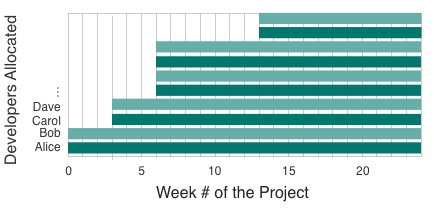
\includegraphics[width=\oneColumnWidth{}]{sustainable_software_development_images/OriginalDeveloperStaffingV3.jpg}
\caption{Planned Developer Staffing}
\label{PlannedDeveloperStaffing}
\end{figure}

The 35-person project consisted of an iOS team of ten engineers, an android team of ten engineers, and a Java back-end team of eight engineers with the support of two to four interaction designers and three product managers. Here we focus on the iOS team. The first iOS release to the Apple store occurred in week 23. Given the success of the project, the client extended the engagement for a second iOS release that happened on week 43. 

Figure \ref{PlannedDeveloperStaffing} shows the staffing plan at the start of Project Quattuor. The plan was to start the project with two developers, while adding more developers as more tracks of work became available. Figure \ref{DeveloperStaffing} shows the actual staffing, which is quite different from the plan.

The bar chart on the top of Figure \ref{DeveloperStaffing} shows when individual developers started and stopped working on the project. Five developers were on the project for most of its duration, while 22 people worked on the project in total. The maximum team size was 12 developers working together at the same time. The graph on the bottom of Figure \ref{DeveloperStaffing} shows the total number of developers allocated to the project at any given week. Developers ramped up from week 5 to week 12, with an average team size of 10 and a maximum of 12 developers.

Developers were routinely rotated and were replaced for various reasons, including promotions, medical leave, leaving the company, transferring to a different office, and vacations. Atypically, the client was more concerned with feature development than cost, so absent developers were replaced, leading to 22 different people working on the same ten-person project. 

The ongoing rotation of team members likely undermined the team’s sense of identity \cite{TuckmanModel}. In addition, the project experienced many challenges, including not having access to production back-end systems or expensive dependent physical components, and cultural differences between Pivotal and the client's deployment organization. Yet the team successfully completed the project. The client was delighted, even claiming that the team delivered a multi-year project in five months by delivering the first release. 

Contrary to conventional wisdom, high team disruption did not appear to negatively influence the success of Project Quattuor. This observation raises our research question: \quotes{How do the observed teams develop software effectively while overcoming team disruption?}


%\begin{figure*}[t]
%\centering
%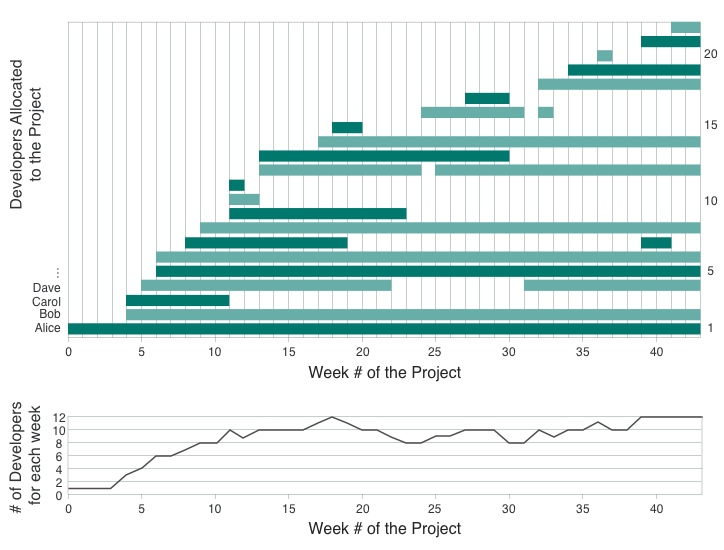
\includegraphics[width=\twoColumnWidth{}]{DeveloperStaffingV4.jpg}
%\caption{Actual Developer Staffing}
%\label{DeveloperStaffing}
%\end{figure*}

\begin{figure}[t]
\centering
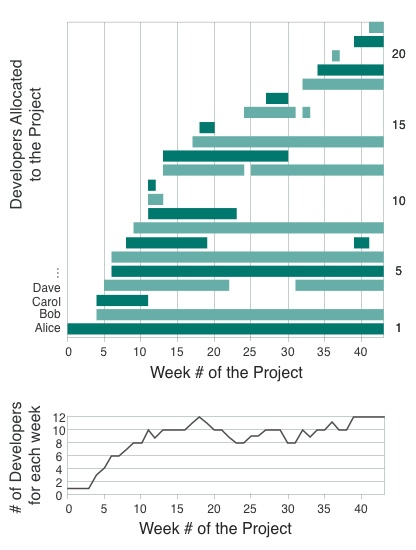
\includegraphics[width=\oneColumnWidth{}]{sustainable_software_development_images/DeveloperStaffingV7.jpg}
\caption{Actual Developer Staffing}
\label{DeveloperStaffing}
\end{figure}

\begin{table*}[t]
\renewcommand{\arraystretch}{1.5}
\centering
\caption{Theory of Sustainable Software Development: Principles, Policies, and Practices}
\label{SustainableSoftwareDevelopmentTable}
\begin{tabular}{|p{1.75in}|p{1.30in}|p{1.75in}|p{1.6in}|}
\hline
\multicolumn{4}{|c|}{\textbf{Sustainable Software Development}} \\
\hline
\textbf{Underlying Principles} & \textbf{Policies} & \textbf{Removing Knowledge Silos Practices} & \textbf{Caretaking the Code Practices} \\
\hline
Engendering Positive Attitudes Toward Team Disruption & Team Code Ownership & Continuous Pair Programming & TDD / BDD \\
Encouraging Knowledge Sharing and Continuity & Shared Schedule & Overlapping Pair Rotation & Continuous Refactoring \\
Caring about Code Quality & Avoid Technical Debt & Knowledge Pollination & Supported by Live on Master \\ 
\hline
\end{tabular}
\end{table*}


\section{Theory of Sustainable Software Development}
\label{Theory}

Sustainable software development refers to the ability and propensity of a software development team to mitigate the negative effects of major disruptions, especially team churn, on its productivity and effectiveness. Our theory of Sustainable Software Development, summarized in Table \ref{SustainableSoftwareDevelopmentTable}, is targeted towards software developers and has emerged from the Grounded Theory research described above. We hypothesize that sustainability emerges from synergistic principles, policies, and practices, which collectively explain how the observed Pivotal teams overcome disruption. The ability of any pair to work on any story while caring about the code is the primary mechanism by which these principles, policies, and practices mitigate disruption. 

In this section, we document each principle, policy, and practice.  For each policy and practice, we present how it is used at Pivotal, and discuss anti-patterns and potential alternatives. We provide deeper descriptions for practices rarely documented in the literature.
\subsection{Principles}

\subsubsection{Engendering Positive Attitudes Toward Disruption}
Conventional wisdom says that team disruption should be avoided. Yet, team disruption is a reality in the industry, as exemplified by Project Quattuor where only five of 22 developers worked on the project for most of its duration (see Figure \ref{DeveloperStaffing}). However, the observed organization engendered a positive attitude towards disruption, transforming a challenge into an opportunity and hence demonstrating remarkable business agility. Team members rolling off the project were replaced as needed. New members rolling onto the project were viewed as an opportunity to improve the current code base by providing a fresh perspective. When a new team member did not understand the code base, he or she revealed issues with code discoverability. New team members often questioned the team’s assumptions and challenged \quotes{cargo culting.} 

The first underlying principle of Sustainable Software Development is engendering an open and positive attitudes towards team disruption, transforming a challenge into an opportunity to improve code quality.

\subsubsection{Encouraging Knowledge Sharing and Continuity}
Despite the fresh perspectives added by new team members, team disruption can precipitate in significant knowledge loss for the organization. Policies and practices that encourage knowledge sharing and continuity mitigate this risk. These policies are Team Code Ownership, and Shared Schedule, while the practices are Continuous Pair Programming, Overlapping Pair Rotation, and Knowledge Pollination (which are discussed below).

The second underlying principle of Sustainable Software Development is encouraging knowledge sharing and continuity, enabling the knowledge to spread from one developer to the next, and eventually reach the entire team. Knowledge sharing and continuity make the team more resistant to disruption. 

\subsubsection{Caring about Code Quality}

Enabling knowledge sharing and continuity does not guarantee sustainable development if the team starts incurring technical debt \cite{McConnellTechnicalDebt}. A set of policy and practices aimed at taking good care of the code itself mitigates this risk. The policy is Avoid Technical Debt, while the practices are Test-Driven Development / Behavior-Driven Development and Continuous Refactoring (which are discussed below).

The third underlying principle of Sustainable Software Development is caring about code quality, hence avoiding technical debt and enabling sustainable team productivity.
\subsection{Policies}

\subsubsection{Team Code Ownership}

\textbf{Description:} Team code ownership is the extent to which any team member can modify any part of the team's code. Code ownership is influenced not only by official policy but also each developer's familiarity with and emotional relationship to the code.

\textbf{Purpose:} Everyone on the team is responsible for the team’s code. Simply saying \quotes{Any team member can modify any piece of the code} is not sufficient to achieve the desired result of team code ownership. We documented five factors that affect the team’s sense of code ownership and eight risks observed on Pivotal teams \cite{SedanoTeamCodeOwnership}. Achieving team code ownership requires a set of enabling practices. These enabling practices aim at removing knowledge silos and taking good care of the code, as described in the following sections.

\textbf{At Pivotal:} Every developer is empowered to work on any part of the team’s code and is encouraged to refactor any code section to improve its quality as needed, especially in cases of low code discoverability and readability.

\textbf{Anti-pattern:} Removing team code ownership makes sustainable software development challenging. Every line of code written via strong ownership might create a knowledge silo. Code reviews are a mitigation strategy with an asynchronous delay. When the delay is too long, merging code onto the master becomes problematic, which discourages Continuous Refactoring. 

\subsubsection{Shared Schedule}
\textbf{Description:} Shared Schedule signifies that all team members have the same work schedule. 

\textbf{Purpose:} Shared Schedule enables Continuous Pair Programming, Overlapping Pair Rotation, and Knowledge Pollination practices. With Shared Schedule, teams form new pairs at the beginning of the day. The evening becomes a natural interruption to the continuous software development workflow. 

\textbf{At Pivotal:} Team members at the Palo Alto office work Monday to Friday from 9:00 am to 6:00 pm. This is done without management coercion; each team member agreed to this fixed schedule to achieve the benefits of Sustainable Software Development. While Shared Schedule is the norm, exceptions are possible. 

Pivotal prefers co-located teams in order to promote synchronous and osmotic communication. Project Quattuor was an exception with the team split between Palo Alto and San Francisco. Each day, developers in one location remotely paired with developers in the other location to spread the knowledge across the two offices.

\textbf{Anti-pattern:} Flexible work hours potentially jeopardizes Continuous Pair Programming, Overlapping Pair Rotation, and Knowledge Pollination practices. A team with flexible work hours might find it difficult to pair program on all stories (as described in the Continuous Pair Programming practice). A team member consistently soloing from 8:00 am to 10:00 am might be building knowledge silos. 

When developers arrive whenever they feel like it, rotating pairs (as described under the Overlapping Pair Rotation practice) becomes awkward, as there is no longer a natural time to rotate pairs. Trying to schedule a time midday to rotate pairs feels artificial. Even if the team says they will rotate later in the day, once pairs get into their stories and form context on what needs to be done, they typically forget about re-pairing until it is time to go home.

Pivotal experimented with pairing when developers arrived, but this meant that developers coming early were making decisions for the team members who arrived later, hence loosing some benefits of pair programming. 

\textbf{Alternatives:} A possible mitigation strategy could be to adopt core work hours. Individuals would solo on simple cleanup chores outside of core hours, and switch to pair programming for feature development when the whole team is in the office. 

\subsubsection{Avoid Technical Debt}
\textbf{Description:} Technical Debt refers to delaying needed technical work, by taking technical shortcuts, usually in pursuit of calendar-driven software schedules \cite{McConnellTechnicalDebt}. 

\textbf{Purpose:} Avoid Technical Debt enables a team to balance feature development with Continuous Refactoring (as described under the Continuous Refactoring practice). When a team is pressured to finish work by a deadline, they might be tempted to focus on feature delivery, take on technical debt, and stop refactoring. When a team delays refactoring and takes on technical debt, the code becomes harder to work with, which in turn makes it more difficult for developers to rotate onto that part of the code base. There is a dialectic tension \cite{RalphProcessTheories} between Continuous Refactoring and delivering more features while accruing technical debt.

\textbf{At Pivotal:} A pair tends to create well-crafted code by avoiding shortcuts and short-term fixes. The team codes for the \quotes{present} by building the simplest solution for the current story. The team eschews over-engineering for potential future features. The team avoids technical debt by building the best solution for the moment at hand. When inheriting a large code base with existing technical debt, we observed a team actively paying down technical debt while delivering new features. 

\textbf{Anti-pattern:} On Project Quattuor, the product manager suggested that the team deliver more stories at the cost of technical debt to make a release date. Some team members followed this suggestion, skipped the refactoring step, and introduced harder to maintain code. This decision made it difficult for pairs to rotate onto parts of the code. Pairs making the decision to skip refactoring caused future pain for the next pair to work with that part of the code. Immediately after the first release, the team spent several weeks refactoring the code to pay down the debt and consistently deliver new features again.
\subsection{Removing Knowledge Silos Practices}
This section presents practices for encouraging knowledge sharing and continuity, enabling the knowledge to spread from one developer to the next, and eventually reach the entire team. This phenomenon is illustrated in Figure \ref{KnowledgeSharing}, where letters A to F represent six developers working in pairs.

\begin{figure}[t]
\centering
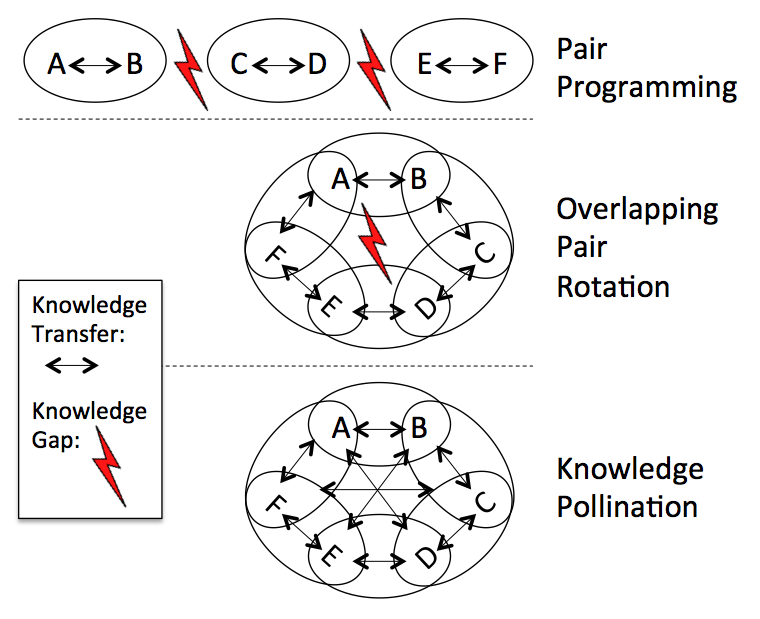
\includegraphics[width=\oneColumnWidth{}]{sustainable_software_development_images/KnowledgeSharingLevels.png}
\caption{Three Levels of Knowledge Sharing}
\label{KnowledgeSharing}
\end{figure}

\subsubsection{Continuous Pair Programming}
\textbf{Description:} Continuous Pair Programming is two developers collaborating to write software together as their normal mode of software development.

\textbf{Purpose:} When two developers work together, they are likely to bring more knowledge, and generate more diverse solutions compared to a solo developer. Additionally, there are many documented benefits of pair programming \cite {Williams2002}. When two developers work together, knowledge spreads from one developer to the next \cite{Zieris2016KnowledgeTransfer}, as illustrated in Figure \ref{KnowledgeSharing}. Overall, pairing reduces knowledge silos and can improve code quality.

\textbf{At Pivotal:} Pairing happens with two monitors, two keyboards, two mice, and one computer. Developers always work in pairs, unless exceptional circumstances arise. For instance, solo programming occurs when one developer is out of the office for part of the day (e.g. at the doctor’s office), out of the office the whole day (e.g. out sick), or involved in another business activity for a few hours (e.g. interviewing candidates, scoping a new project). When solo programming, developers take low-risk chores, refactorings, or stories. With any sizable project, there usually is something the team has been meaning to do that one person can safely do and report back to the team on its completion. 

\textbf{Anti-pattern:} Removing this practice results in solo programming where there is a clear owner for the code written. This would increase individual ownership and start creating knowledge silos. 

\textbf{Alternatives:} In solo programming, to remove silos, developers could take the stories for the part of the code they know least about. Assigning stories to developers who have the least understanding of the code could be a hard sell to management as it reduces productivity (at least initially). Bird \cite{BirdDontTouchMyCode} suggests that this approach would introduce more defects. 

\subsubsection{Overlapping Pair Rotation}
\textbf{Description:} Overlapping Pair Rotation happens when there is a rotation of the people working on a track of work: one developer rolls off the track and another developer rolls on, keeping continuity of one developer at each rotation. This results in knowledge continuity for a track of work, as illustrated in Figure \ref{KnowledgeSharing}. Typically, rotations happen in the morning as the evenings provide a natural interruption to the work. 

\textbf{Purpose:} The rotation of developers helps spread knowledge and promotes team code ownership. The goal is to prevent the situation where one or two developers understands how  part of the system works and must be assigned any story related to that part of the system. The entire team should be able to modify the code. Rotation helps prevent knowledge silos and individual code ownership from forming. 

\textbf{At Pivotal:} Whenever a knowledge silo begins to emerge, the team actively fights against it and tries to spread that knowledge around through pair rotation. During the study, three strategies were observed.

\textit{Optimizing for people rotation:} Most teams rotate based on who has paired with whom. Developers try to pair with the person they \quotes{least recently paired with} (basically a Least Recently Used strategy). Some teams use rotation techniques or tools to track this information.

This strategy does not clearly articulate the purpose of knowledge silo removal and the need for knowledge transfer. As an example, developers who recently left a track of work might ask to be rotated back without realizing the potential cost to the team. This prevents an opportunity to spread the knowledge to the rest of the team. (This issue is more serious on larger teams; on a four person team, this is not an issue).

\textit{Optimizing for personal preferences:} A few teams allow developers to pick with whom they will work or on which stories to work based on individual preferences. This has the same downsides as the previous strategy. 

\textit{Optimizing for context sharing:} A few teams are experimenting with rotating onto a track the person who has not been working on the track for the longest time. The goal each day is for the developer leaving the track next to empower the developer who will remain on the track. Before any rotation, the remaining developer is asked, \quotes{Was enough context shared with you?} If the answer is no, then the first developer does not leave and the pair continues to work together for another day. This provides a feedback loop on how well the team is transferring knowledge. 

\textbf{Anti-pattern:} Removing this practice means that developers can work on the same part of the code base for extended periods of time, developing individual code ownership and knowledge silos. One participant described their experience at a previous company that follows Extreme Programming. Developers could be paired for more than a month working on only one part of the system. This lack of pair rotation led to deep knowledge silos. 

Ideally, developers work on the next, non-blocked story at the top of the backlog. When developers start skipping down the backlog, it can be an indication that they might not have enough context to work on any story. On Project Quattuor, a knowledge silo emerged around a complicated bug related to an obsolete technology that only a handful of people understood. Often developers would skip over stories and bugs related to that technology. At one point, the product manager reminded the team to keep \quotes{working from the top of backlog.}

Sometimes a developer wants to see a story through to completion over multiple days. Maybe he or she enjoys the technology or the feature. In these situations, agreeing to the request may result in forming knowledge silos and creating a sense of personal ownership. Statements like \quotes{We need Marion on that story, only she really knows the Apple watch code base,} or \quotes{Shea knows the ins-and-outs of the legacy integration, we need him to work on this story,} suggest that knowledge silos have emerged. 

\textbf{Alternatives:} Team members that build a knowledge silo can share what they learned through a demo, code walk through, or a team huddle. This helps a team share knowledge, but is less effective than working directly with the code. 

\subsubsection{Knowledge Pollination}
\textbf{Description:} Knowledge Pollination refers to the set of activities contributing to knowledge sharing in an unstructured way. Examples include daily stand-up meetings, weekly retrospections, writing or sketching on whiteboards, overhearing a conversation, using the backlog to communicate current status about a story, calling out an update to the entire team, or simply reaching out to others to ask questions as needed. 

\textbf{Purpose:} Knowledge Pollination contributes to spreading knowledge among the team as illustrated in Figure \ref{KnowledgeSharing}.

\textbf{At Pivotal:} Daily standups create awareness of who is working on what. Teams can write down a \quotes{parking lot} of issues to discuss during daily standups. A pair may record the current status of a blocked story so that the next pair picking it up knows the situation. Osmotic communication helps when a developer overhears another pair discussing an issue and offers needed knowledge. Instead of thrashing, a pair interrupts another pair to gain the needed information. Thus, interruptions are encouraged because they make the entire team more efficient as knowledge pollinates across the team. 

Calling out an update to the entire team might be a simple as shouting \quotes{The build is broken, we are looking into it}, or this interchange: \quotes{We just checked in a presenter,} followed by \quotes{We just used your presenter. That’s great collaboration.}

While working on a story, a pair may discover that they are missing some key context that prevents them from efficiently proceeding. If the issue is about the acceptance criteria for a story, they clarify with the product manager. If the issue is about the code base, the pair can ask the people who recently worked on that section of code, or ask the entire team. To determine whom to ask, the pair may remember who did what at stand-up, look through Pivotal Tracker (an agile project management tool) to see who worked on a story, or check out source code version history (e.g. git annotate). Two-, four-, and six- person teams seem to have collective memory of who worked on which features from daily standup. 

These mechanisms help a team build awareness. Chong observed that \quotes{transmission of awareness information is a relatively effortless act in the XP environment} in her ethnographic study comparing an Extreme Programming team to a traditional team \cite{ChongNominum}.
 
\textbf{Anti-pattern:} An organization that provides little opportunity to share knowledge leads to wasted time as developers must acquire the knowledge through other means or end up reinventing the wheel.
\subsection{Caretaking the Code Practices}
\subsubsection{Test-Driven Development, Behavior-Driven Development}
\textbf{Description:} In Test-Driven Development (TDD) developers write unit tests before creating a design and writing code. In Behavior-Driven Development (BDD) developers implement acceptance tests before creating a design and writing code. Most lines of production code are tested before the production code is written. The software’s design emerges from the tests and subsequent refactorings.

In Extreme Programming, Kent Beck describes his corresponding \quotes{Testing} practice as developers writing \quotes{automated unit tests} and implementing customer provided \quotes{functional tests} for story acceptance \cite{BeckExtremeProgramming1999}. Later, he refines these ideas as \quotes{Test-first programming} \cite{BeckExtremeProgramming2004}. 

\textbf{Purpose:} This practice creates a safety net and empowers a pair to have the confidence to modify the code base. This enables any pair to pick up any story. Continuous Refactoring results in easier to modify tests.

\textbf{At Pivotal:} Developers use a combination of TDD and BDD. While each project is different, programmers tend to use BDD to describe interactions between the user and the system and TDD at a unit test level. Teams use a variety of TDD strategies including testing the responsibilities and interactions \cite{Goose} or contract testing using mocks \cite{RainsbergerIntegrationTestsYouTube}. In Pivotal’s ideal, the design emerges from the creation and exploration of the test cases. 

\textbf{Anti-pattern:} Without this testing practice, developers no longer have the confidence to change any part of the code as they may unknowingly end-up breaking something else. 

\textbf{Alternatives:} For a system without a test suite documenting the system specification, a possible remedy is for developers to own particular parts of the system in order to understand the ramifications of changes. Creating strong code ownership and knowledge silos is exactly the problem that sustainable software development is trying to solve.

Writing tests after the code is written could produce a safety net for refactoring, provided that tests correctly exercise the system. (A test that never failed might not be testing anything). We did not observe this behavior and future research is necessary to determine if any testing approach is sufficient for sustainable software development.

\subsubsection{Continuous Refactoring}
\textbf{Description:} Continuous Refactoring is the systematic improvement of the code base concurrently with new feature development. When developers identify something wrong such as a code smell, they simply fix it. In this regard, developers are caretaking the code by continuously improving it. This practice results in an emergent software design, as well as empathy for the code as developers learn to \quotes{listen to the code.} 

%Continuous Refactoring is one way to prevent technical debt from accumulating. When a team employs continuous refactoring, the team refines a code base towards simple design, intention revealing code, and discoverable code. 

\textbf{Purpose:} Continuous Refactoring enables any pair to work on any part of the system. Long-term benefits for the team include increased code discoverability, code readability, code modifiability, and code simplicity. 

\textbf{At Pivotal:} Developers typically do some refactoring while implementing stories. Developers are encouraged to improve the code’s design, make the code easier to understand, and increase the discoverability of a component based on its responsibility. Usually, the team prefers \quotes{pre-factoring} where the developer does the complicated work to make the implementation of the current story as simple and easy as possible, as opposed to \quotes{post-factoring} where refactoring happens after the story is done, but before it is delivered. 

\textbf{Anti-pattern:} Removing this practice might produce difficult to modify and messy code. Developers might not be able to easily work on any part of the code base. When refactoring is skipped, code might be simply bolted on to the existing design. Soon it becomes increasingly difficult to bolt more code on. A dilemma arises for the programmers working on the next story: do they continue bolting on more code, or do they perform the pretermitted refactorings? Removing this practice may also result in hard-to-change tests.

\textbf{Alternatives:} Postponing refactoring may be necessary in extreme situations, for instance, when the company might go out of business unless the company releases the next version. In such situations, the team risks taking on uncontrolled technical debt as \quotes{refactoring later} turns into \quotes{refactoring never.} 

\subsubsection{Live on Master}
\textbf{Description:} Live on master means that developers integrate their code several times a day, as quickly as possible. ExtremeProgramming.org calls this practice \quotes{Integrate Often} \cite{WellsIntegrateOften}.

\textbf{Purpose:} For teams to continuously refactor and minimize the waste of merge conflicts, the entire team needs to routinely merge their code onto master. If a pair communicates to the team that they are actively \quotes{refactoring} a component, they are asserting exclusive temporary ownership over the file to avoid merge conflicts. While this is a normal practice for a few hours, if it happens for multiple days, the team is losing collective ownership of that code. The team is not able to receive any of the benefits until the work is merged back to master. 

\textbf{At Pivotal:} In the ideal workflow, developers merge their code to master many times a day. If a pair has not merged to master by the afternoon, the pair typically starts examining why this is difficult and explores ways of incrementally making changes. Developers may use branches to save spikes. When rotating pairs, developers may use branches to move work-in-progress code between machines. 

\textbf{Anti-pattern:} Removing this practice means that code lives in branches for days or weeks. Integrations might be painful due to merge conflicts and developers might delay needed refactorings. If a developer has code only on their machine, then no one else on the team can use or modify that code. When code lives only on one machine for many days in a row, the machine acts as a \quotes{virtual branch.} Running a Continuous Integration box and having long running branches is an anti-pattern.
\section{Theory Evaluation}
\label{TheoryEvaluation}

Charmaz identifies four criteria for evaluating a Grounded Theory: credibility (\quotes{Is there sufficient data to merit claims?}), originality (\quotes{Do the categories offer new insights?}), resonance (\quotes{Does the theory make sense to participants?}), and usefulness (\quotes{Does the theory offer useful interpretations?}) \cite{StolGroundedTheory}. 

\textbf{Credibility:} The current data set is rich and its analysis leads to theory saturation. (Saturation means that the properties of the theory are complete and are not affected by new data.) The data set comprises 21 intensive interviews conducted in four different offices, field notes from participant observation on Project Quattuor, and the first author’s involvement in four other projects as participant-observer.

\textbf{Originality:} The theory uniquely depicts the principles, policies, and practices enabling software development sustainability in an organization. Since the organization under study follows Extreme Programming, it is not surprising that many of the practices of Sustainable Software Development are defined in Extreme Programming. However, overlapping pair rotation and its supporting principles, policies, and practices are central and unique to the proposed theory.

\textbf{Resonance:} The participants examined the theory. The theory resonates with their experience and reflects the way they work.

\textbf{Usefulness:} The theory informs Pivotal engineers as to why Pivotal purposefully avoids knowledge silos, and how the theory’s principles, policies, and practices work together to accomplish the team’s goals. The theory explains why the principles, policies, and practices should be incorporated together. A few managers use  the theory to help potential clients understand how Pivotal achieves the business goals of both the client and Pivotal.

\section{Threats to Validity}

\subsection{External Validity}

\textbf{Generalizability across situations:} Grounded Theory does not support statistical generalization from a sample to a population. The results may not be applicable to other teams or other domains. There are four broad types of scientific generalization: 1) from data to descriptions, 2) from descriptions to concepts, 3) from concepts to theory, 4) from theory to description \cite{Lee2003generalizing}. Grounded Theory research involves the first three kinds of generalization. Generalizing from a theory tested in one context to descriptions of a new context (the fourth kind of generalization) could be done by the researchers in the new context, on a case-by-case basis. However, we have not attempted to perform any type four generalizations at this time.

\subsection{Internal Validity}
\textbf{Researcher bias:} A risk of the participant-observer technique is that the researcher may lose perspective and become biased by being a member of the team. An outside observer might see something the researcher missed. We mitigated this risk by recording interviews and with a colleague reviewing the coding process.

\textbf{Prior knowledge bias:} With Grounded Theory, prior knowledge can aid the researcher in looking at interesting research questions or create difficulties by blinding the researcher about possible explanations \cite{GlaserIssues}. We mitigated this risk with a colleague reviewing the coding process. 
\section{Future Research}
We are interested in the tension between individual and team ownership, as well as the factors that foster and decrease the sense of ownership. Developers, interaction designers, and product managers all have different goals for their role. In future work, we plan to examine how the sense of ownership is driven by different factors for each role.

Some programmers naturally adapt to team code ownership, while others struggle with the transition. Future research could follow new Pivotal engineers and examine their journey in transitioning from individual code ownership to team code ownership. Perhaps there are 
specific practices that Pivotal or the development team could employ to ease the transition. We could also investigate the optimal team size for team code ownership, or explore whether Sustained Software Development works for a distributed team with a Shared Schedule.
\section{Conclusions}
This paper introduces a descriptive theory of \quotes{Sustainable Software Development} as a solution to the challenge of software development sustainability for an ever changing workforce. The theory emerged from a Constructivist Grounded Theory research study. By collecting data from 21 intensive interviews conducted in four different Pivotal offices, field notes from participant-observation on the Project Quattuor, and the first author’s involvement in four other Pivotal projects as participant-observer, the study investigates the research question \quotes{How do the observed teams develop software effectively while overcoming team disruption?}

The emergent theory is characterized by a collection of synergistic principles, policies, and practices encouraging a positive attitude towards team disruption, knowledge sharing and continuity, as well as caring about code quality. The theory refines and extends Extreme Programming by adding principles, policies, and practices (including Overlapping Pair Rotation) and aligning them with the business goal of sustainability.

Conventional wisdom says that team disruptions should be avoided, and that extensive documentation is needed to prevent knowledge loss during team churn. Unfortunately, documentation often quickly becomes out-of-date and unreliable. The theory positions team code ownership with overlapping pair rotation and knowledge pollination as an alternative and potentially more effective strategy to mitigate against knowledge loss.

The primary benefits to the software developer are the ability to understand the entire system, the ability to work on every story, increased in teaching opportunities to share one’s expertise, and more nuanced understanding of the utilized technologies. 

The primary benefit to the employer is business agility. The engineering team continues to deliver software week after week, month after month, while surviving cataclysmic events. Things do not fall apart when the superstar developer leaves because features or components are not critically tied to a particular individual. Critical feature work can be parallelized since anyone can work on any feature.  The whole team’s talents are leveraged.


\appendices
\section{Proof of the First Zonklar Equation}
Appendix one text goes here.

% you can choose not to have a title for an appendix
% if you want by leaving the argument blank
\section{}
Appendix two text goes here.

\section*{Acknowledgments}
Thank you to Rob Mee, David Goudreau, Ryan Richard, and Zach Larson for making this research possible. Thank you to Karina Sils for creating Figure \ref{PlannedDeveloperStaffing} and Figure \ref{DeveloperStaffing} using Sketch.

\ifCLASSOPTIONcaptionsoff
  \newpage
\fi

\bibliographystyle{IEEEtran}
\bibliography{bibliography} 

\begin{IEEEbiography}{Todd Sedano}
Biography text here.
\end{IEEEbiography}

% if you will not have a photo at all:
\begin{IEEEbiographynophoto}{Paul Ralph}
Biography text here.
\end{IEEEbiographynophoto}

\begin{IEEEbiography}{Paul Ralph}
Biography text here.
\end{IEEEbiography}

\begin{IEEEbiography}{C\'ecile P\'eraire}
Biography text here.
\end{IEEEbiography}
























































\begin{table*}[t]
\renewcommand{\arraystretch}{1.5}
\centering
\caption{Sample Quotes}
\label{ChainOfEvidenceTable}
\begin{tabular}{|p{1.65in}|p{5.55in}|}
\hline
\multicolumn{2}{|c|}{Underlying Principles} \\
\hline
\textbf{Engendering Positive Attitudes Toward Team Disruption} & \\
& \participantQuote{I'm excited when a new person joins the team. That person has experience that might add something to the project.} \\

& \participantQuote{I like that people bring new energy. Projects often get into the state of a lull with the same people working on it and have the same cadence. New people bring a new perspective. [Two engineers recently joined] and it was really cool to see their fresh perspective. I always like people joining a project.} \\

& \participantQuote{There's all this shared knowledge and context that is in our team culture. It is invisible to us. [Adding another person exposes it to the team.]}  \\
 & \participantQuote{You get an outsider’s perspective. They bring a fresh set of eyes.} \\

& \participantQuote{The team is extremely welcoming. I was surprised to see that there was no \quotes{us} versus \quotes{them} between developers and product.}  \\

\hline
Encouraging Knowledge Sharing and Continuity & Example 1b \\
& \participantQuote{[When pairing], we discuss the change through, and what we want to do. We make decisions after our discussions. [At the end of the track], it’s everybody’s decision who has touched this code. It’s really hard for me say that [any particular piece] was my idea. [Even still], I feel that I own that codebase.} \\

& \participantQuote{We managed to preserve [team code ownership] even though it’s a big team and we had many people rotating on and off  the project.  We still had a team effort and the team owned the entire codebase.} \\

& \participantQuote{I have a general sense of confidence around the codebase. Given any story in the backlog, I’m reasonably confident that I could start it and figure it out.} \\

& \participantQuote{It is important to enable other programmers to quickly know the responsibility of each component and control flow.} \\

& \participantQuote{My ideal team size is two pairs. Anything that we did today, by tomorrow, the team will have an opportunity to know what we’ve done.  After one rotation, context is shared immediately throughout the team.} \\

& \participantQuote{Everyone has context about the entire system, and everyone's constantly communicating about the entire system.} \\

\hline
Caring about Code Quality & Example 1c \\

& \participantQuote{Everyone is responsible for fixing issues and everyone can fix it.} \\
& \participantQuote{We should encourage the feeling that since I can change anything, I need to make sure all the code I write and come across is good. } \\
& \participantQuote{It is important to create a culture of \quotes{it is ok to make a mistake.}} \\
& \participantQuote{I feel pretty good about the product and the code base.  We did a lot of good work and implemented many features.} \\
\hline
\end{tabular}
\end{table*}




\begin{table*}[t]
\renewcommand{\arraystretch}{1.5}
\centering
\caption{Sample Quotes}
\label{ChainOfEvidenceTable}
\begin{tabular}{|p{1.65in}|p{5.55in}|}
\hline
\multicolumn{2}{|c|}{Policies} \\
\hline
\textbf{Team Code Ownership} & Example 2a \\
& \participantQuote{I feel ownership of it as a whole and that I feel like I’m empowered and able to like go on and work on any part of the codebase.} \\
& \participantQuote{I don’t feel like I have [individual] ownership. It’s really a collaborative effort to achieve where we are today \ldots I feel like everybody owns this product.} \\
& \participantQuote{There is a lot of emphasis that you are not your code.} \\
& \participantQuote{I never feel like a specific piece is mine or something belongs to other people.}\\
& \participantQuote{Hey this is our code.} \\
& \participantQuote{I feel the freedom to make changes as I see necessary. It’s always a discussion with [my pair]. We come to a conclusion on what we want to do next.} \\
& \participantQuote{I felt like that had my thumbprint on it on the clay.} \\
& \participantQuote{I think we should encourage the feeling of ownership as in I can change anything and this is all mine.} \\ 
& \participantQuote{It is worth having everyone being able to do anything.} \\

\hline
Shared Schedule & Example 2b \\
\hline

Avoid Technical Debt & Example 2c \\
& One participant described his feelings about the code, \participantQuote{I am proud and disgusted by the code.} When asked to explain the disgusted side, the participant said, \participantQuote{We have dug ourselves into technical debt holes several times and then that combined with the time pressure means that like we keep putting it off \ldots I found myself shying away from those parts of the system. I feel less ownership over that part of the code now.} \\
& Caretaking the code by making it better and cleaning up messes. \participantQuote{Sometimes I kind of feel like a janitor to [the code base]. Maybe caretaker would be better. Yeah, probably caretaker. I feel like a janitor just cleans up messes, but a caretaker makes things better.} \\
& \participantQuote{Things that I build can be subsequently removed.} \\
& \participantQuote{Code structure is clean.} \\
& \participantQuote{We are pretty good at separating all the logics in specific classes. I think that our codebase is pretty flexible. When we want to do refactors, it’s not super complicated and not super hard to do.} \\
& Thinking \quotes{someone else} will do a refactor or solve a problem means that nobody will do it. \participantQuote{Thinking that someone else will do it can be dangerous, because if everybody thinks that, then nobody will do it.} \\
\hline
\end{tabular}
\end{table*}




\begin{table*}[t]
\renewcommand{\arraystretch}{1.5}
\centering
\caption{Sample Quotes}
\label{ChainOfEvidenceTable}
\begin{tabular}{|p{1.65in}|p{5.55in}|}
\hline
\multicolumn{2}{|c|}{Removing Knowledge Silos Practices} \\
\hline
Continuous Pair Programming &
Example 3a \\
\hline
\textbf{Overlapping Pair Rotation} & Example 3b \\

& \participantQuote{To make sure that knowledge silos don’t form we rotate pairs. As people work on specific stories and specific parts of the code, we want to share that knowledge.} \\

& \participantQuote{Rotating pairs reduces knowledge silos and reduces the bus factor. We do not want to the departure of one developer from the project to cripple the project.} \\


& \participantQuote{We rotate pairs because everyone has a different set of knowledge. When you work with someone you get a little bit of that knowledge. The more you pair with them, the more knowledge you get.} \\

& \participantQuote{My ideal team size is two pairs. Anything that we did today, by tomorrow, the team will have an opportunity to know what we’ve done.  After one rotation, context is shared immediately throughout the team.} \\

& On one project ūnus, one developer kept the story with everyone else rotating through. After day four, that developer was annoyed that the anchor wanted to refactor \quotes{everything} the team had created. By maintaining continuity on the story, the developer had built strong individual code ownership. \\

& Overlapping Pair Rotation helps spread context through the team. One developer said, 
\participantQuote{I have a general sense of confidence around the codebase. Given any story in the backlog, I’m reasonably confident that I could go and figure it out.} When knowledge silos emerged, we saw reluctance to pick up certain stories. Some developers wanted to only work with the knowledge experts on those stories which then further entrenched the knowledge expert at the expert. A team employing the \textit{Optimizing for context sharing} strategy would prevent one team member from building a knowledge silo. \\

& \participantQuote{At the beginning of the day, I might keep the story or roll off of it and join another story with somebody else already working on it.} \\

& In describing his experience at another Extreme Programming software company, one participant said, \participantQuote{Actually I paired with him for three weeks. I then paired with two weeks [before the holidays] and again throughout the four weeks in January \ldots There were infrequent rotations of pairs except in the event of personality conflicts.} This led to building of deep knowledge silos. The pairs would specifically only work in one part of the code base, and would not be able to easily work in other parts of the code base. \\

& Working on the same track decreases empowering to change anything in the code base. \participantQuote{Yeah, I’d be more hesitant to work on other people’s modules. I mean I’d be less empowered to go fix other things. As a result, I feel the code would turn into a lot of very orderly pieces that are connected in terrible ways. I wouldn’t feel as much ownership over the whole codebase.} \\

& With a big team, keeping shared context is challenging as so much parallel work is being done. \participantQuote{I feel that we don’t have context spread around fully but then again having five, sometimes six pairs on the project makes it go really fast so it’s hard to keep context \ldots It is a big team and you can be working on one track for a week perhaps and then the other four pairs move fast. Things just change under you. You get back to some other place and you’re saying \quotes{oh what happened here.} Because of that speed, it’s harder to keep context on everything. } \\
\hline
Knowledge Pollination & Example 3c \\
\hline
\end{tabular}
\end{table*}




\begin{table*}[t]
\renewcommand{\arraystretch}{1.5}
\centering
\caption{Sample Quotes}
\label{ChainOfEvidenceTable}
\begin{tabular}{|p{1.65in}|p{5.55in}|}
\hline
\multicolumn{2}{|c|}{Caretaking the Code Practices} \\
\hline
TDD / BDD & Example 4a \\
\hline
Continuous Refactoring & Example 4b \\
\hline
& In describing the project’s code, the developer said, \participantQuote{It was really easy to do refactoring on the code that we want to modify. So, I guess the code is pretty flexible.} It was desirable for the team to create code that was easy to modify since this allowed future developers to understand and modify the code. \\
& Continuous Refactoring helped developers create components with clear separation of concerns.  One developer said, \participantQuote{[It is easy] to know what objects I need to modify \ldots it really allows me to change things without breaking everything else \ldots they are pretty separated.}  On these projects, Continuous Refactoring helped the developers to know where to find the classes responsible for a particular concern, e.g. the discoverability of code. \\

\hline
Supported by Live on Master & Example 4c \\
&  \participantQuote{We have a preferred way of doing software development that works, things like frequent commits and always rebasing.} \\
& Pivots try to commit and push multiple times a day. In the afternoon, if they have not pushed, they tend to get \quotes{impatient} and begin to look to ways to commit sooner. \\
& On one project, one machine had  multiple commits from several days without integrating to master (almost like a virtual branch). The pair working on that machine asked the team to not change parts of the system since it would result in merge conflicts. Other members of the team inquired about the nature of the work to see if it could be decomposed into incremental refactors. These could be routinely integrated as opposed to one \quotes{big bang} integration. \\
& Several Pivotal Data product teams are open source projects. All of their work is submitted to master via a pull request. This makes everyone work the same way, just like open source contributors outside the organization. The pull request system makes it hard to do refactors. There is a delay from when the code is submitted to when it is merged into master. Since master may have changed, merge conflicts ensue. This discourages the team from doing refactoring and they rarely refactor.  \\
& One engineer described his experience at a previous company that used pull requests. The review often took more than a week. The code changed so much that it no longer was feasible to merge back into master. The engineer would give up with trying to integrate it, use it as a reference implementation, and re-write the change on the current code from scratch. \\
\hline
\end{tabular}
\end{table*}






%
% paper title
% Titles are generally capitalized except for words such as a, an, and, as,
% at, but, by, for, in, nor, of, on, or, the, to and up, which are usually
% not capitalized unless they are the first or last word of the title.
% Linebreaks \\ can be used within to get better formatting as desired.
% Do not put math or special symbols in the title.
% \title{Bare Demo of IEEEtran.cls for\\ IEEE Computer Society Journals}
%
%
% author names and IEEE memberships
% note positions of commas and nonbreaking spaces ( ~ ) LaTeX will not break
% a structure at a ~ so this keeps an author's name from being broken across
% two lines.
% use \thanks{} to gain access to the first footnote area
% a separate \thanks must be used for each paragraph as LaTeX2e's \thanks
% was not built to handle multiple paragraphs
%
%
%\IEEEcompsocitemizethanks is a special \thanks that produces the bulleted
% lists the Computer Society journals use for "first footnote" author
% affiliations. Use \IEEEcompsocthanksitem which works much like \item
% for each affiliation group. When not in compsoc mode,
% \IEEEcompsocitemizethanks becomes like \thanks and
% \IEEEcompsocthanksitem becomes a line break with idention. This
% facilitates dual compilation, although admittedly the differences in the
% desired content of \author between the different types of papers makes a
% one-size-fits-all approach a daunting prospect. For instance, compsoc 
% journal papers have the author affiliations above the "Manuscript
% received ..."  text while in non-compsoc journals this is reversed. Sigh.

% \author{Michael~Shell,~\IEEEmembership{Member,~IEEE,}
%         John~Doe,~\IEEEmembership{Fellow,~OSA,}
%         and~Jane~Doe,~\IEEEmembership{Life~Fellow,~IEEE}% <-this % stops a space
% \IEEEcompsocitemizethanks{\IEEEcompsocthanksitem M. Shell was with the Department
% of Electrical and Computer Engineering, Georgia Institute of Technology, Atlanta,
% GA, 30332.\protect\\
% % note need leading \protect in front of \\ to get a newline within \thanks as
% % \\ is fragile and will error, could use \hfil\break instead.
% E-mail: see http://www.michaelshell.org/contact.html
% \IEEEcompsocthanksitem J. Doe and J. Doe are with Anonymous University.}% <-this % stops an unwanted space
% \thanks{Manuscript received April 19, 2005; revised August 26, 2015.}}

% note the % following the last \IEEEmembership and also \thanks - 
% these prevent an unwanted space from occurring between the last author name
% and the end of the author line. i.e., if you had this:
% 
% \author{....lastname \thanks{...} \thanks{...} }
%                     ^------------^------------^----Do not want these spaces!
%
% a space would be appended to the last name and could cause every name on that
% line to be shifted left slightly. This is one of those "LaTeX things". For
% instance, "\textbf{A} \textbf{B}" will typeset as "A B" not "AB". To get
% "AB" then you have to do: "\textbf{A}\textbf{B}"
% \thanks is no different in this regard, so shield the last } of each \thanks
% that ends a line with a % and do not let a space in before the next \thanks.
% Spaces after \IEEEmembership other than the last one are OK (and needed) as
% you are supposed to have spaces between the names. For what it is worth,
% this is a minor point as most people would not even notice if the said evil
% space somehow managed to creep in.



% The paper headers
% \markboth{Journal of \LaTeX\ Class Files,~Vol.~14, No.~8, August~2015}%
% {Shell \MakeLowercase{\textit{et al.}}: Bare Demo of IEEEtran.cls for Computer Society Journals}
% The only time the second header will appear is for the odd numbered pages
% after the title page when using the twoside option.
% 
% *** Note that you probably will NOT want to include the author's ***
% *** name in the headers of peer review papers.                   ***
% You can use \ifCLASSOPTIONpeerreview for conditional compilation here if
% you desire.



% The publisher's ID mark at the bottom of the page is less important with
% Computer Society journal papers as those publications place the marks
% outside of the main text columns and, therefore, unlike regular IEEE
% journals, the available text space is not reduced by their presence.
% If you want to put a publisher's ID mark on the page you can do it like
% this:
%\IEEEpubid{0000--0000/00\$00.00~\copyright~2015 IEEE}
% or like this to get the Computer Society new two part style.
%\IEEEpubid{\makebox[\columnwidth]{\hfill 0000--0000/00/\$00.00~\copyright~2015 IEEE}%
%\hspace{\columnsep}\makebox[\columnwidth]{Published by the IEEE Computer Society\hfill}}
% Remember, if you use this you must call \IEEEpubidadjcol in the second
% column for its text to clear the IEEEpubid mark (Computer Society jorunal
% papers don't need this extra clearance.)



% use for special paper notices
%\IEEEspecialpapernotice{(Invited Paper)}



% for Computer Society papers, we must declare the abstract and index terms
% PRIOR to the title within the \IEEEtitleabstractindextext IEEEtran
% command as these need to go into the title area created by \maketitle.
% As a general rule, do not put math, special symbols or citations
% in the abstract or keywords.
% \IEEEtitleabstractindextext{%
% \begin{abstract}
% The abstract goes here.
% \end{abstract}

% Note that keywords are not normally used for peerreview papers.
% \begin{IEEEkeywords}
% Computer Society, IEEE, IEEEtran, journal, \LaTeX, paper, template.
% \end{IEEEkeywords}}


% % make the title area
% \maketitle


% To allow for easy dual compilation without having to reenter the
% abstract/keywords data, the \IEEEtitleabstractindextext text will
% not be used in maketitle, but will appear (i.e., to be "transported")
% here as \IEEEdisplaynontitleabstractindextext when the compsoc 
% or transmag modes are not selected <OR> if conference mode is selected 
% - because all conference papers position the abstract like regular
% papers do.
% \IEEEdisplaynontitleabstractindextext
% \IEEEdisplaynontitleabstractindextext has no effect when using
% compsoc or transmag under a non-conference mode.



% For peer review papers, you can put extra information on the cover
% page as needed:
% \ifCLASSOPTIONpeerreview
% \begin{center} \bfseries EDICS Category: 3-BBND \end{center}
% \fi
%
% For peerreview papers, this IEEEtran command inserts a page break and
% creates the second title. It will be ignored for other modes.
% \IEEEpeerreviewmaketitle



% \IEEEraisesectionheading{\section{Introduction}\label{sec:introduction}}
% Computer Society journal (but not conference!) papers do something unusual
% with the very first section heading (almost always called "Introduction").
% They place it ABOVE the main text! IEEEtran.cls does not automatically do
% this for you, but you can achieve this effect with the provided
% \IEEEraisesectionheading{} command. Note the need to keep any \label that
% is to refer to the section immediately after \section in the above as
% \IEEEraisesectionheading puts \section within a raised box.




% The very first letter is a 2 line initial drop letter followed
% by the rest of the first word in caps (small caps for compsoc).
% 
% form to use if the first word consists of a single letter:
% \IEEEPARstart{A}{demo} file is ....
% 
% form to use if you need the single drop letter followed by
% normal text (unknown if ever used by the IEEE):
% \IEEEPARstart{A}{}demo file is ....
% 
% Some journals put the first two words in caps:
% \IEEEPARstart{T}{his demo} file is ....
% 
% Here we have the typical use of a "T" for an initial drop letter
% and "HIS" in caps to complete the first word.
% \IEEEPARstart{T}{his} demo file is intended to serve as a ``starter file''
% for IEEE Computer Society journal papers produced under \LaTeX\ using
% IEEEtran.cls version 1.8b and later.
% You must have at least 2 lines in the paragraph with the drop letter
% (should never be an issue)
% I wish you the best of success.

% \hfill mds
 
% \hfill August 26, 2015

% \subsection{Subsection Heading Here}
% Subsection text here.

% needed in second column of first page if using \IEEEpubid
%\IEEEpubidadjcol

% \subsubsection{Subsubsection Heading Here}
% Subsubsection text here.


% An example of a floating figure using the graphicx package.
% Note that \label must occur AFTER (or within) \caption.
% For figures, \caption should occur after the \includegraphics.
% Note that IEEEtran v1.7 and later has special internal code that
% is designed to preserve the operation of \label within \caption
% even when the captionsoff option is in effect. However, because
% of issues like this, it may be the safest practice to put all your
% \label just after \caption rather than within \caption{}.
%
% Reminder: the "draftcls" or "draftclsnofoot", not "draft", class
% option should be used if it is desired that the figures are to be
% displayed while in draft mode.
%
%\begin{figure}[!t]
%\centering
%\includegraphics[width=2.5in]{myfigure}
% where an .eps filename suffix will be assumed under latex, 
% and a .pdf suffix will be assumed for pdflatex; or what has been declared
% via \DeclareGraphicsExtensions.
%\caption{Simulation results for the network.}
%\label{fig_sim}
%\end{figure}

% Note that the IEEE typically puts floats only at the top, even when this
% results in a large percentage of a column being occupied by floats.
% However, the Computer Society has been known to put floats at the bottom.


% An example of a double column floating figure using two subfigures.
% (The subfig.sty package must be loaded for this to work.)
% The subfigure \label commands are set within each subfloat command,
% and the \label for the overall figure must come after \caption.
% \hfil is used as a separator to get equal spacing.
% Watch out that the combined width of all the subfigures on a 
% line do not exceed the text width or a line break will occur.
%
%\begin{figure*}[!t]
%\centering
%\subfloat[Case I]{\includegraphics[width=2.5in]{box}%
%\label{fig_first_case}}
%\hfil
%\subfloat[Case II]{\includegraphics[width=2.5in]{box}%
%\label{fig_second_case}}
%\caption{Simulation results for the network.}
%\label{fig_sim}
%\end{figure*}
%
% Note that often IEEE papers with subfigures do not employ subfigure
% captions (using the optional argument to \subfloat[]), but instead will
% reference/describe all of them (a), (b), etc., within the main caption.
% Be aware that for subfig.sty to generate the (a), (b), etc., subfigure
% labels, the optional argument to \subfloat must be present. If a
% subcaption is not desired, just leave its contents blank,
% e.g., \subfloat[].


% An example of a floating table. Note that, for IEEE style tables, the
% \caption command should come BEFORE the table and, given that table
% captions serve much like titles, are usually capitalized except for words
% such as a, an, and, as, at, but, by, for, in, nor, of, on, or, the, to
% and up, which are usually not capitalized unless they are the first or
% last word of the caption. Table text will default to \footnotesize as
% the IEEE normally uses this smaller font for tables.
% The \label must come after \caption as always.
%
%\begin{table}[!t]
%% increase table row spacing, adjust to taste
%\renewcommand{\arraystretch}{1.3}
% if using array.sty, it might be a good idea to tweak the value of
% \extrarowheight as needed to properly center the text within the cells
%\caption{An Example of a Table}
%\label{table_example}
%\centering
%% Some packages, such as MDW tools, offer better commands for making tables
%% than the plain LaTeX2e tabular which is used here.
%\begin{tabular}{|c||c|}
%\hline
%One & Two\\
%\hline
%Three & Four\\
%\hline
%\end{tabular}
%\end{table}


% Note that the IEEE does not put floats in the very first column
% - or typically anywhere on the first page for that matter. Also,
% in-text middle ("here") positioning is typically not used, but it
% is allowed and encouraged for Computer Society conferences (but
% not Computer Society journals). Most IEEE journals/conferences use
% top floats exclusively. 
% Note that, LaTeX2e, unlike IEEE journals/conferences, places
% footnotes above bottom floats. This can be corrected via the
% \fnbelowfloat command of the stfloats package.




% \section{Conclusion}
% The conclusion goes here.





% if have a single appendix:
%\appendix[Proof of the Zonklar Equations]
% or
%\appendix  % for no appendix heading
% do not use \section anymore after \appendix, only \section*
% is possibly needed

% use appendices with more than one appendix
% then use \section to start each appendix
% you must declare a \section before using any
% \subsection or using \label (\appendices by itself
% starts a section numbered zero.)
%


% \appendices
% \section{Proof of the First Zonklar Equation}
% Appendix one text goes here.

% % you can choose not to have a title for an appendix
% % if you want by leaving the argument blank
% \section{}
% Appendix two text goes here.


% % use section* for acknowledgment
% \ifCLASSOPTIONcompsoc
%   % The Computer Society usually uses the plural form
%   \section*{Acknowledgments}
% \else
%   % regular IEEE prefers the singular form
%   \section*{Acknowledgment}
% \fi


% The authors would like to thank...


% Can use something like this to put references on a page
% by themselves when using endfloat and the captionsoff option.
% \ifCLASSOPTIONcaptionsoff
%   \newpage
% \fi



% trigger a \newpage just before the given reference
% number - used to balance the columns on the last page
% adjust value as needed - may need to be readjusted if
% the document is modified later
%\IEEEtriggeratref{8}
% The "triggered" command can be changed if desired:
%\IEEEtriggercmd{\enlargethispage{-5in}}

% references section

% can use a bibliography generated by BibTeX as a .bbl file
% BibTeX documentation can be easily obtained at:
% http://mirror.ctan.org/biblio/bibtex/contrib/doc/
% The IEEEtran BibTeX style support page is at:
% http://www.michaelshell.org/tex/ieeetran/bibtex/
%\bibliographystyle{IEEEtran}
% argument is your BibTeX string definitions and bibliography database(s)
%\bibliography{IEEEabrv,../bib/paper}
%
% <OR> manually copy in the resultant .bbl file
% set second argument of \begin to the number of references
% (used to reserve space for the reference number labels box)

% \bibliographystyle{IEEEtran}
% \bibliography{bibliography} 


% \begin{thebibliography}{1}

% \bibitem{IEEEhowto:kopka}
% H.~Kopka and P.~W. Daly, \emph{A Guide to \LaTeX}, 3rd~ed.\hskip 1em plus
%   0.5em minus 0.4em\relax Harlow, England: Addison-Wesley, 1999.

% \end{thebibliography}

% biography section
% 
% If you have an EPS/PDF photo (graphicx package needed) extra braces are
% needed around the contents of the optional argument to biography to prevent
% the LaTeX parser from getting confused when it sees the complicated
% \includegraphics command within an optional argument. (You could create
% your own custom macro containing the \includegraphics command to make things
% simpler here.)
%\begin{IEEEbiography}[{\includegraphics[width=1in,height=1.25in,clip,keepaspectratio]{mshell}}]{Michael Shell}
% or if you just want to reserve a space for a photo:

% \begin{IEEEbiography}{Todd Sedano}
% Biography text here.
% \end{IEEEbiography}

% % if you will not have a photo at all:
% \begin{IEEEbiographynophoto}{Paul Ralph}
% Biography text here.
% \end{IEEEbiographynophoto}

% \begin{IEEEbiography}{Paul Ralph}
% Biography text here.
% \end{IEEEbiography}

% \begin{IEEEbiography}{C\'ecile P\'eraire}
% Biography text here.
% \end{IEEEbiography}


% insert where needed to balance the two columns on the last page with
% biographies
%\newpage

% \begin{IEEEbiographynophoto}{Jane Doe}
% Biography text here.
% \end{IEEEbiographynophoto}

% You can push biographies down or up by placing
% a \vfill before or after them. The appropriate
% use of \vfill depends on what kind of text is
% on the last page and whether or not the columns
% are being equalized.

%\vfill

% Can be used to pull up biographies so that the bottom of the last one
% is flush with the other column.
%\enlargethispage{-5in}



% that's all folks
\end{document}


